\documentclass[fleqn,10pt]{wlscirep}
\usepackage{fixltx2e}
\usepackage{epstopdf}

\newcommand{\beginsupplement}{%
 \setcounter{table}{0}
 \renewcommand{\thetable}{S\arabic{table}}%
 \setcounter{figure}{0}
 \renewcommand{\thefigure}{S\arabic{figure}}%
 }

\title{Dendritic cells isolated from individuals susceptible to tuberculosis have an altered gene expression profile}


\author[1,2]{John D. Blischak}
\author[3]{Ludovic Tailleux}
\author[1]{Marsha Myrthil}
\author[4,5,*]{Luis B. Barreiro}
\author[1,*]{Yoav Gilad}



\affil[1]{Department of Human Genetics, University of Chicago, Chicago, Illinois, USA}
\affil[2]{Committee on Genetics, Genomics, and Systems Biology, University of Chicago, Chicago, Illinois, USA}
\affil[3]{Mycobacterial Genetics Unit, Institut Pasteur, Paris, France}
\affil[4]{Department of Genetics, CHU Sainte-Justine Research Center, Montreal, Québec, Canada}
\affil[5]{Department of Pediatrics, University of Montreal, Montreal, Québec, Canada}



\affil[*]{Correspondence should be addressed to YG (gilad@uchicago.edu) and LBB (luis.barreiro@umontreal.ca).}


\begin{abstract}
Write abstract here…
\end{abstract}
\begin{document}
\flushbottom
\maketitle
\thispagestyle{empty}

\section*{Introduction}

\section*{Results}

\subsection*{Susceptible individuals have an altered transcriptome in the noninfected state}

We obtained whole blood samples from 25 healthy individuals. Six of the donors had recovered from a previous active TB infection, and are thus susceptible. The remaining 19 tested positive for a latent TB infection without ever experiencing symptoms of active TB, and are thus resistant. We isolated dendritic cells (DCs) and treated them with \emph{Mycobacterium }\emph{tuberculosis} (MTB) or a mock control. To measure genome-wide gene expression levels, we sequenced the RNA at 18 hours post-infection, using a processing pipeline designed to minimize the introduction of unwanted technical variation, and obtained a mean of X $\pm$ X million raw reads per sample. We performed quality control analyses to remove non-expressed genes (Supplementary Fig. \ref{fig:gene}), identify and remove outliers (Supplementary Fig. \ref{fig:outliers}), and check for confounding batch effects (Supplementary Fig. \ref{fig:batch}, \ref{fig:infection}). Ultimately 6 samples were removed from all downstream analyses (Supplementary Fig. \ref{fig:outliers}).

Next we performed a standard differential expression analysis using a linear modeling framework, defined in equation (\ref{eq:limma}). Of most interest are genes which were differentially expressed (DE) between susceptible and resistant individuals in the noninfected and infected states (Fig. \ref{fig:limma}). After correcting for multiple testing, we identified X DE genes in the noninfected state, and none in the infected state. <Insert GO results and a few examples>

\begin{figure}[p]
\centering
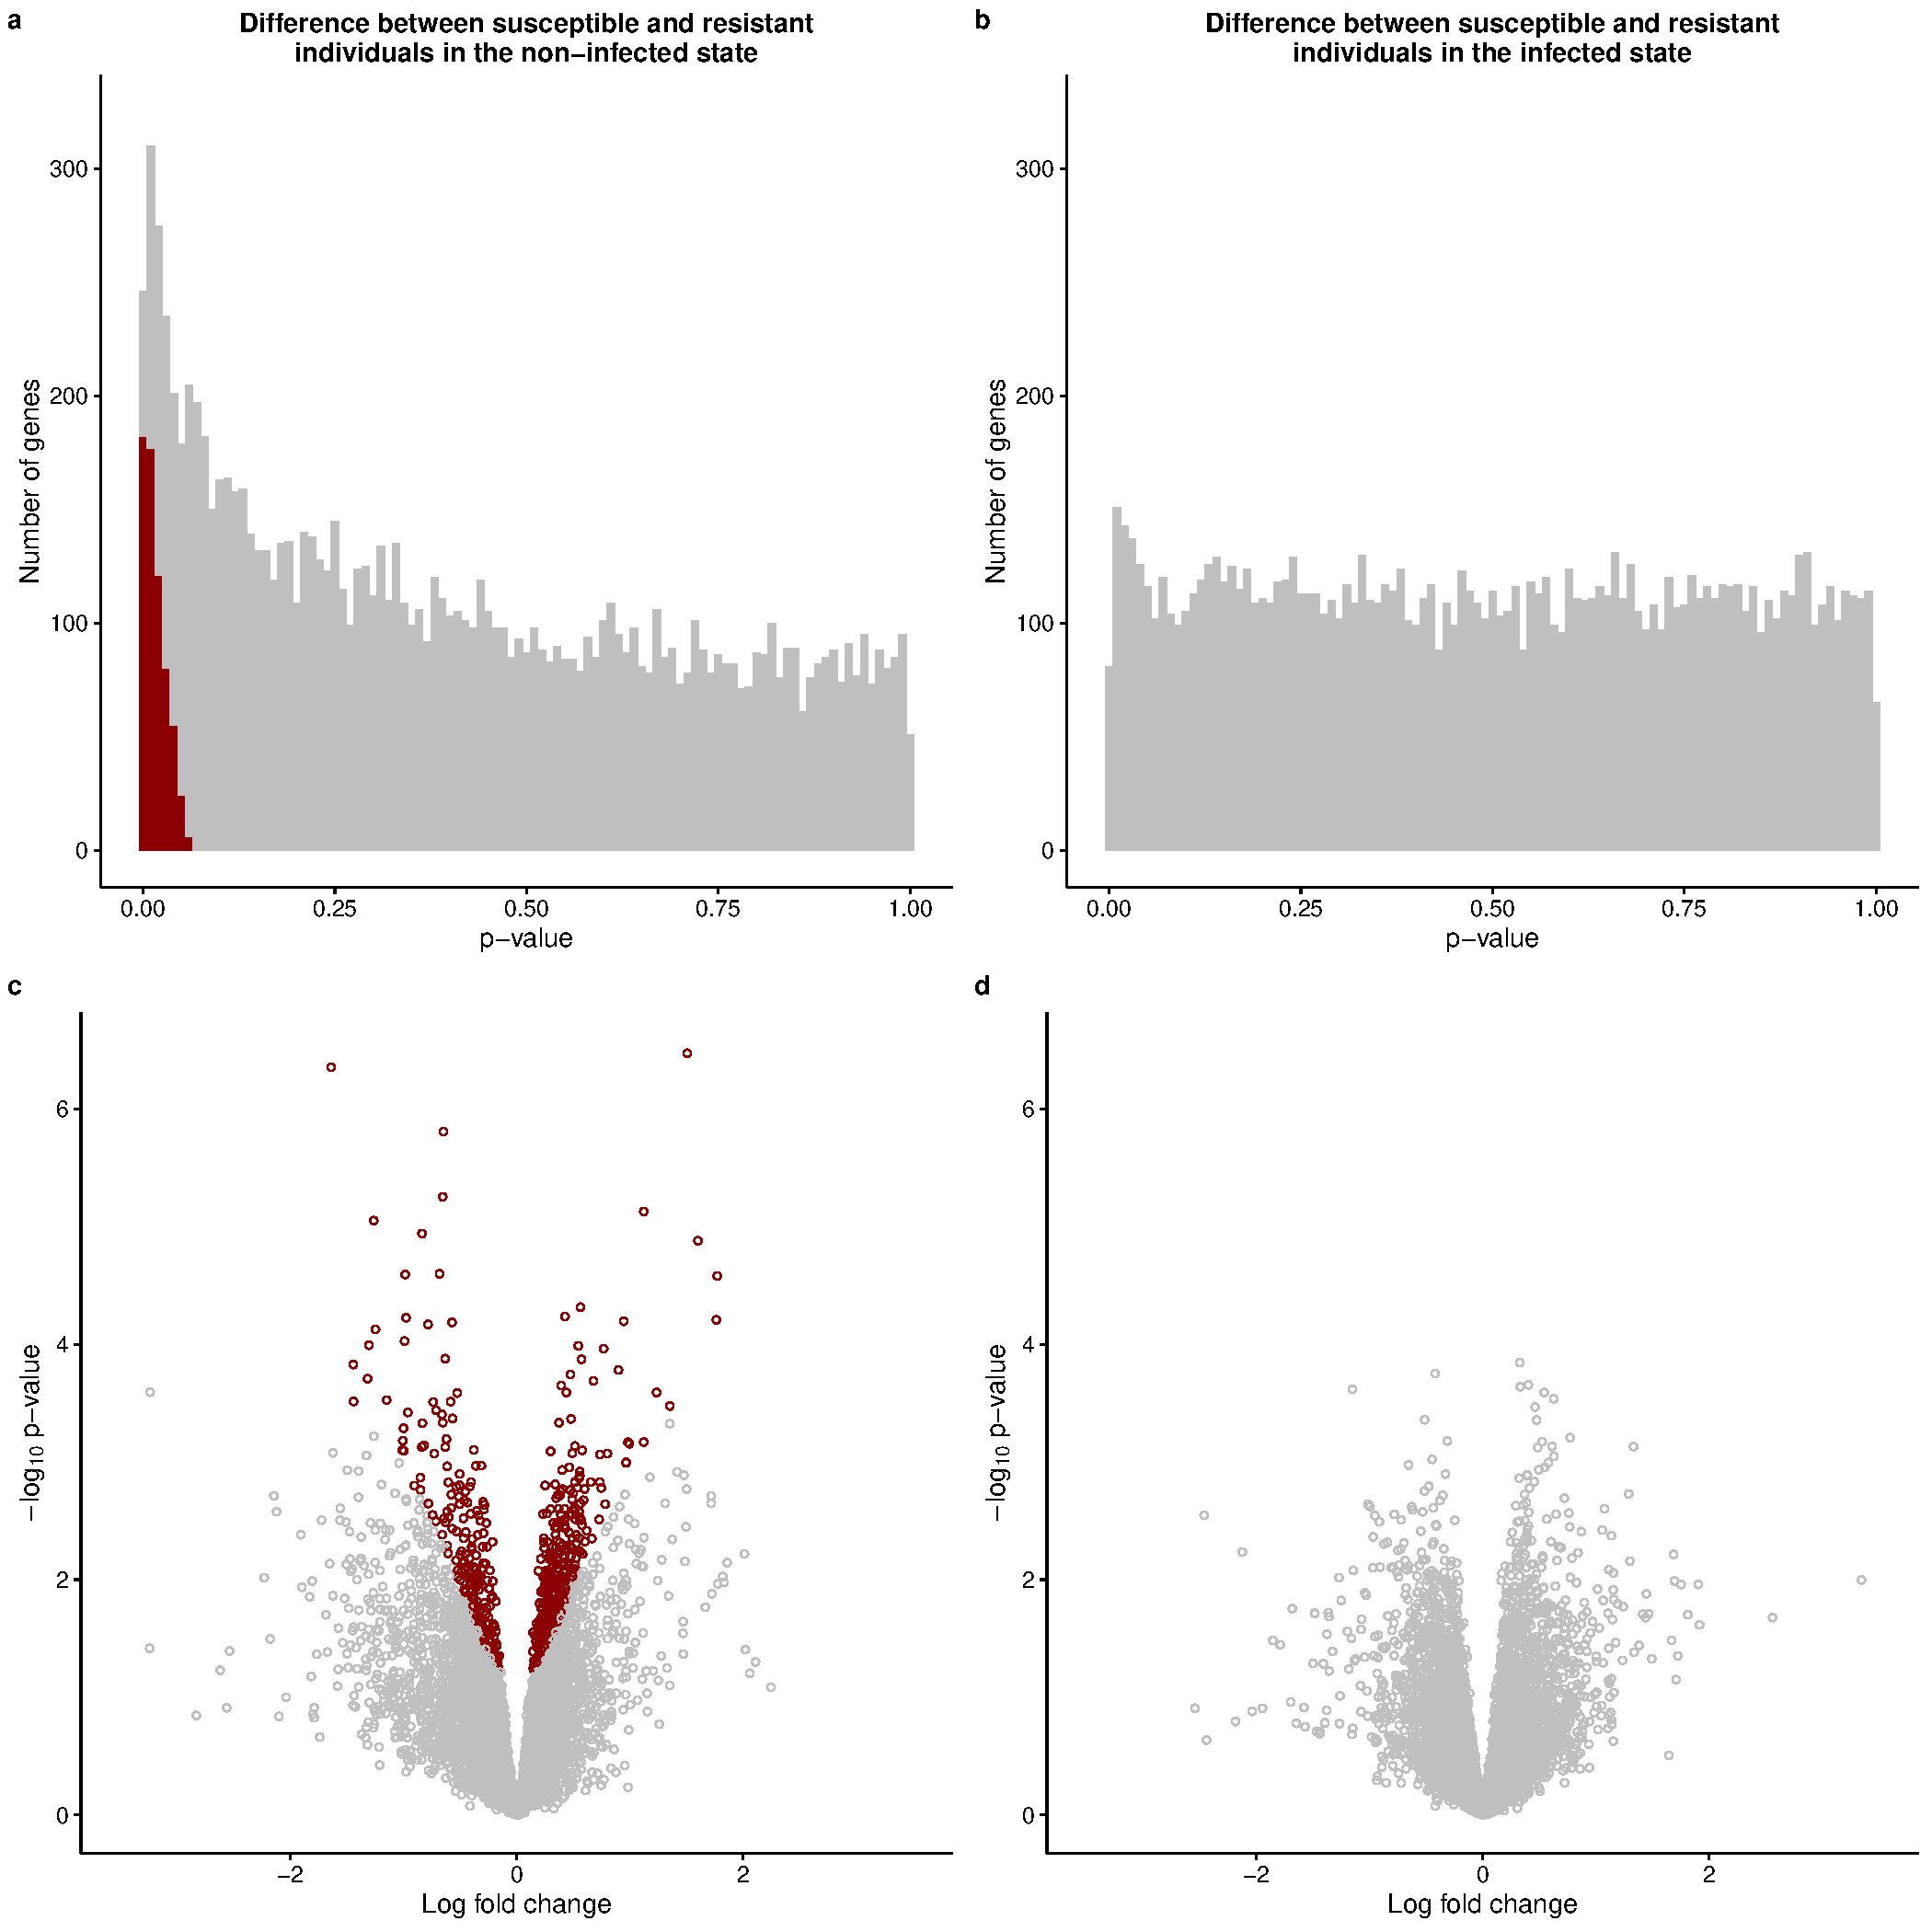
\includegraphics[width=\linewidth]{../figure/limma.pdf}
\caption{
Differential expression analysis. The top panel contains the distribution of unadjusted p-values after testing for differential expression between susceptible and resistant individuals in the (a) noninfected or (b) infected state. The bottom panel contains the corresponding MA plots for the (c) noninfected and (d) infected states. The x-axis is the average gene expression level and the y-axis is the log fold change in expression level between susceptible and resistant individuals. Red solid dots indicate genes which are significant differentially expressed after applying a multiple testing correction.
}
\label{fig:limma}
\end{figure}
\subsection*{Differentially expressed genes are enriched for TB susceptibility loci}

We next sought to investigate whether the differentially expressed genes we had identified in our \emph{in vitro} experimental system were important for the genetic basis of TB susceptibility. To do this, we compared our results to a TB susceptibility GWAS conducted in Gambia and Ghana \cite{Thye2010}. Specifically, for each gene we assigned the SNP with the lowest p-value among all SNPs located within 50 kb of its transcription start site (TSS). If the differentially expressed genes are enriched for TB susceptibility loci, we expect a negative correlation between the absolute values of the log fold changes in our experiment and the GWAS p-values. Indeed, this is what we observed (results from Gambia GWAS in Fig. \ref{fig:gwas}, results from Ghana GWAS in Supplementary Fig. \ref{fig:ghana}). We fit a best fit linear line using least squares regression for each of our differential expression tests. Interestingly, we observed the steepest negative slopes for the tests comparing differential expression between susceptible and resistant individuals in the noninfected or infected states (Fig. \ref{fig:gwas}b). However, the slopes of the best fit lines for the tests of the effect of treatment in either resistant or susceptible individuals was were also negative. Reassuringly, we did not observe a negative relationship between the GWAS p-values and the mean expression levels (in fact it this had a positive slope). Therefore the negative slopes we observed were not an artifact due to the power to call differential expression in our experimental system.

\begin{figure}[ht]
\centering
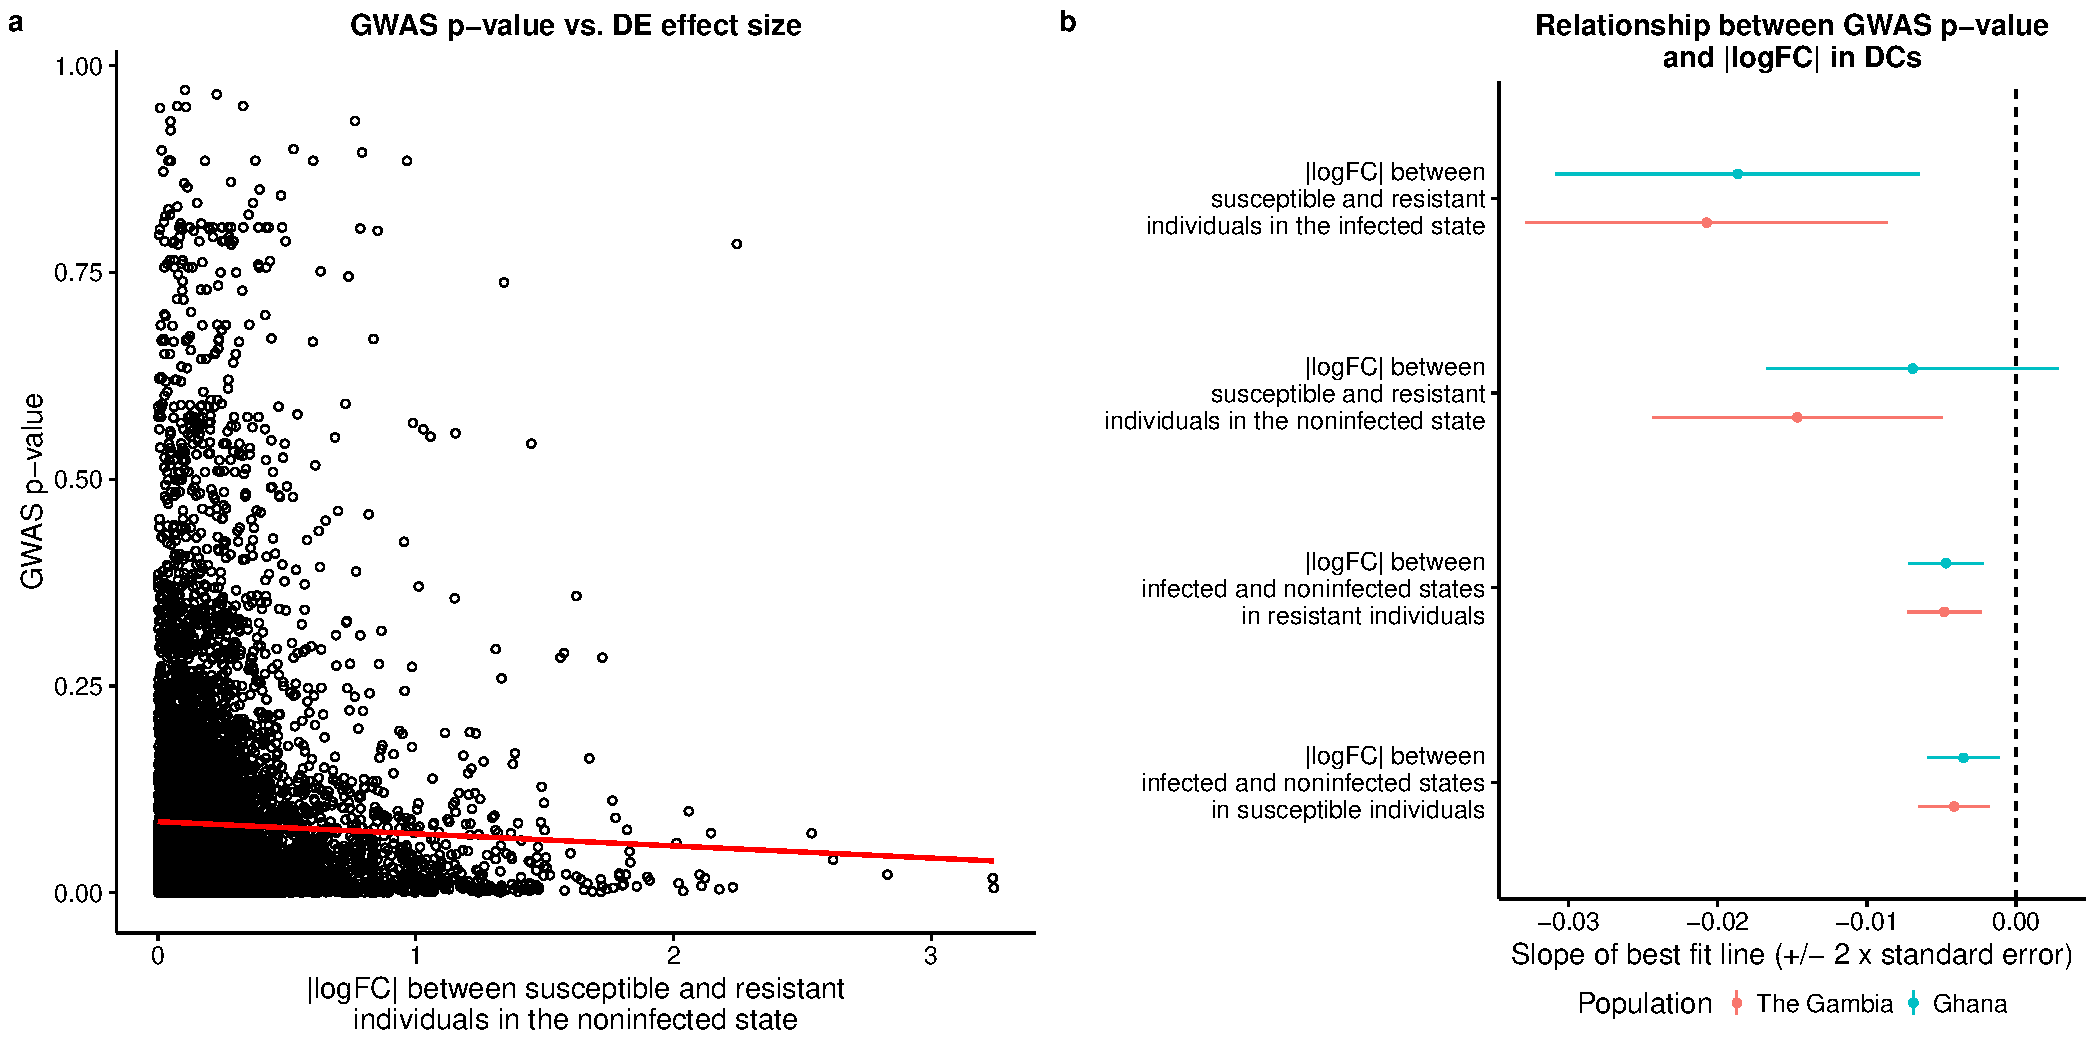
\includegraphics[width=\linewidth]{../figure/gwas.pdf}
\caption{
Comparison of differential expression and GWAS results. (a) The relationship between GWAS p-values \cite{Thye2010} and the absolute values of the log fold changes between susceptible and resistant individuals in the noninfected state. The red line is the least squares regression. (b) The slopes ($\pm$ standard error) of the regression lines for each test. Additionally it includes the comparison of the mean expression level to the GWAS p-values as a control. All slopes are significantly different than 0 (F-test \emph{P} $<$ 0.05).
}
\label{fig:gwas}
\end{figure}

\subsection*{Gene expression levels in the noninfected state can predict susceptibility status}

Next we attempted to build a gene expression based classifier to predict susceptibility status. We focused on the gene expression levels both because this is where we observed the largest differences between susceptible and resistant individuals (Fig. \ref{fig:limma}ac) and also since it is much more practical to obtain gene expression data from noninfected DCs compared to MTB-infected DCs. We trained an elastic net classifier using the 1,057 genes that were differentially expressed at an ASH s-value \cite{Stephens2016} less than 5\%, using leave-one-out-cross-validation to select the optimal model parameters. Encouragingly, we observed a clear separation between susceptible and resistant individuals when comparing the predicted probability of being resistant to TB for each sample obtained from the cross validation (Fig. \ref{fig:classifier}). Using a cutoff of 0.8 for the predicted probability of being resistant to TB infection, we obtained a sensitivity of 100\% (5 out of 5 susceptible individuals labeled as susceptible) and a specificity of ~71\% (5 out of 7 individuals classified as susceptible were true positives).

Unfortunately our current data set was too small to properly split into separate training and testing sets. In order to assess the plausibility of our model, we applied the classifier to an independent study which collected genome-wide gene expression levels in DCs from 65 healthy individuals \cite{Barreiro2012}. Using the same cutoff of 0.8 for the probability of being resistant to TB that was determined to be optimal in the training set, ~9\% (6 out of 65) of the individuals were classified as being susceptible to TB, similar to the general estimate that 10\% of the population is susceptible to TB (Fig. \ref{fig:classifier}).

\begin{figure}[ht]
\centering
%\includegraphics[width=\linewidth]{../figure/classifier.pdf}
\caption{
Classifying TB susceptible individuals. (left) The  estimates of predicted probability of TB resistance from the leave-one-out-cross-validation for individuals in the current study. The red open circles represent individuals known to be susceptible to TB. The horizontal blue line at a probability of 0.8 separates susceptible and resistant individuals. (right) The estimates of predicted probability of TB resistance from applying the classifier trained on the data from the current study to a test set of independently collected healthy individuals \cite{Barreiro2012}.
}
\label{fig:classifier}
\end{figure}

\section*{Discussion}

We obtained dendritic cells (DCs) from individuals that were known to be susceptible or resistant to developing active tuberculosis (TB) and measured genome-wide gene expression levels 18 hours post-infection with \emph{Mycobacterium tuberculosis} (MTB) and noninfected controls. Interestingly, we identified X genes which were differentially expressed between susceptible and resistant individuals in the noninfected state, including X, Y, and Z (Fig. \ref{fig:limma}. Furthermore, we found that these differentially expressed genes were enriched for low GWAS p-values (Fig. \ref{fig:gwas}) and could be used to classify susceptible and resistant individuals. 

Previous work in TB \cite{Thuong2008}
Previous work using gene expression to understand susceptibility \cite{Bryant2014}

Overall our promising results in this small study suggest that collecting blood samples from a larger cohort of susceptible individuals would enable building a gene expression based classifier able to confidently assess risk of TB susceptibility. By reducing the number of resistant individuals receiving treatment for a latent TB infection, we can eliminate the adverse health effects of a 6 month regimen of antibiotics for these individuals and also reduce the selective pressures on MTB to develop drug resistance.
\section*{Methods}

\subsection*{Sample collection}

We collected whole blood samples from healthy Caucasian male individuals living in France. The putatively resistant individuals tested positive for a latent TB infection in an interferon-$\gamma$ release assay, but had never developed active TB. The putatively sensitive individuals had developed active TB in the past, but were currently healthy. Our protocol was approved by the Institutional Review Boards of the University of Chicago (10-504-B) and the Institut Pasteur (IRB00006966).
\subsection*{Isolation and infection of dendritic cells}


\subsection*{RNA extraction and sequencing}

We extracted RNA using the Qiagen miRNeasy Kit and prepared sequencing libraries using the Illumina TruSeq Kit. We sent the master mixes to the University of Chicago Functional Genomics Facility to be sequenced on an Illumina HiSeq 4000. We designed the batches for RNA extraction, library preparation, and sequencing to balance the experimental factors of interest and thus avoid potential technical confounders.
\subsection*{Read mapping}

We mapped reads to human genome hg38 (GRCh38) using Subread and discarded non-uniquely mapping reads. We downloaded the exon coordinates of 19,800 Ensembl protein-coding genes (Ensembl 83, Dec 2015, GRCh38.p5) using the R/Bioconductor package biomaRt and assigned mapped reads to these genes using featureCounts.
\subsection*{Quality control}

First we filtered genes by their expression level by removing all genes with a median log\textsubscript{2} counts per million (cpm) less than zero. This resulted in a final set of 11,336 genes for downstream analysis (Supplementary Fig. \ref{fig:gene}). Next we used principal components analysis (PCA) and hierarchical clustering to identify and remove 6 outliers (Supplementary Fig. \ref{fig:heat-all}, \ref{fig:heat-filt}, \ref{fig:outliers}). We did this systematically by removing any sample that did not fall within the mean $\pm$ two standard deviations from the mean value of the first six PCs. Furthermore, for the first PC which separated the samples by treatment, we calculated a separate mean for the noninfected and infected samples.

After filtering lowly expressed genes and removing outliers, we recalculated the PCA to check for any potential confounding technical batch effects (Supplementary Fig. \ref{fig:batch}). Reassuringly, the major sources of variation in the data were from the biological factors of interest. PC1 was strongly correlated with the effect of treatment, and PCs 2-6 were correlated with inter-individual variation. The only concerning technical factor was the infection experiments, which were done in 12 separate batches. Infection batch correlated with PCs 3 and 5; however, we verified that this variation was not confounded with our primary outcome of interest, TB susceptibility (Supplementary Fig. \ref{fig:infection}).
\subsection*{Differential expression analysis}

We used limma+voom \cite{Smyth2004, Law2014, Ritchie2015} to implement the following linear model to test for differential expression:
\begin{equation} \label{eq:limma}
Y\ \sim \beta_{0} + X_{treat}\beta_{treat} + X_{status}\beta_{status} + X_{treat,status}\beta_{treat,status} + I + \epsilon
\end{equation}
where $\beta_{0}$ is the mean expression level in noninfected cells of resistant individuals, $\beta_{treat}$ is the fixed effect of treatment in resistant individuals, $\beta_{status}$ is the fixed effect of susceptibility status in noninfected cells, $\beta_{treat,status}$ is the fixed effect of treatment in susceptible individuals, and $I$ is the random effect of individual. The random individual effect was implemented using the limma function duplicateCorrelation (cite paper). To jointly model the data with voom and duplicateCorrelation, we followed the recommended best practice of running both voom and duplicateCorrelation twice in succession.

We used the model to test 4 separate hypotheses. We identified genes which were differentially expressed between infected and noninfected DCs of resistant individuals by testing $\beta_{treat} = 0$, genes which were differentially expressed between infected and noninfected DCs of susceptible individuals by testing $\beta_{treat} + \beta_{treat,status} = 0$, genes which were differentially expressed between susceptible and resistant individuals in the noninfected state by testing $\beta_{status} = 0$, and genes which were differentially expressed between susceptible and resistant individuals in the infected state by testing $\beta_{status} + \beta_{treat,status} = 0$. We corrected for multiple testing using the adaptive shrinkage (ash) approached implemented in ashr (). An alternative to traditional false discovery rate (FDR) methods, ash is an empirical Bayesian method that estimates whether an observed effect size was assigned the correct sign (termed the local false sign rate) instead of attempting to estimate whether an observed effect size is different from zero \cite{Stephens2016}. We report differentially expressed genes as those with an s-value below 10\%, analogous to a 10\% q-value cutoff.
\subsection*{Comparison to GWAS results}

The GWAS p-values were from a study conducted in the Gambia and Ghana populations \cite{Thye2010}. To compare our differential expression results to these genetic associations, we assigned each gene the p-value of the SNP with the minimum p-value out of all the SNPs located within 50 kb up or downstream of its transcription start site. Specifically, we obtained the genomic coordinates of the SNPs with the R/Bioconductor package SNPlocs.Hsapiens.dbSNP144.GRCh38 and matched SNPs to nearby genes using GenomicRanges. X of the Y were assigned an association p-value. For each of the 4 hypotheses we tested, we performed least squares regression of the differential expression effect sizes (the log fold changes) and the assigned GWAS p-values. We assessed the statistical significance of these regressions using the standard F-test and reported the slope of each regression line (Fig. \ref{fig:gwas} for the Gambia GWAS; Supplementary Fig. X for the Ghana GWAS).
\subsection*{Classifier}

The training set included the X noninfected samples from this study with known susceptibility status. The test set included the 65 noninfected samples from one of our previous studies in which the susceptibility status is unknown, and thus assumed to be similar to that in the general population ($\sim 10\%$) \cite{Barreiro2012}. Because the two studies are substantially different, we took multiple steps to make them comparable. First, we subset to include only those X genes which were assayed in both. Second, because the dynamic range obtained from RNA-seq (current study) and microarrays (previous study \cite{Barreiro2012}) are very different, we normalized the gene expression levels to a standard normal with $\mu = 0$ and $\sigma = 1$ (Supplementary Fig. SX). Third, we corrected for the large, expected batch effect between the two studies by regressing out the first principal component of the combined expression data using the limma function removeBatchEffect \cite{Ritchie2015} (Supplementary Fig. SX).

To identify genes to use in the classifier, we performed a differential expression analysis on the normalized, batch-corrected data from the current study using the same approach described above (with the exception that we no longer used voom since the data were no longer counts). We tested for differential expression between susceptible and resistant individuals in the noninfected state and identified X genes at an s-value of 5\%. We used the R package caret (cite) to train an elastic net regression classifer (cite glmnet) and chose the model parameters using the kappa statistic. We reported the probability of being TB resistant for each sample in the training set using the estimate from leave-one-out-cross-validation (Fig. \ref{fig:classifier}a). We tested the classifier by predicting the probability of being TB resistant in the 65 healthy samples (Fig. \ref{fig:classifier}b).
\subsection*{Software implementation}

We automated our analysis using Python and Snakemake cite. Our processing pipeline used the general bioinformatics software FastQC, MultiQC, samtools, and bioawk. We used R for all statistics and data visualization. The computational resources were provided by the University of Chicago Research Computing Center. All code is available for viewing and reuse at https://github.com/jdblischak/tb-suscept.
\subsection*{Data availability}

\section*{Acknowledgements}

We thank T. Thye for sharing the GWAS data with us. This study was funded by National Institutes of Health (NIH) Grant AI087658 to YG and LT. JDB was supported by NIH T32GM007197. The content is solely the responsibility of the authors and does not necessarily represent the official views of the NIH.
\section*{Author Contributions}

YG, LT, and LBB conceived of the study and designed the experiments. LT performed the infection experiments. MM extracted the RNA and prepared the sequencing libraries. JDB analyzed the results. LBB and YG supervised the project. JDB and YG wrote the original draft. All authors reviewed the manuscript.

\bibliography{references}


\clearpage\newpage
\beginsupplement
\section*{Supplementary Information}

\subsection*{Supplementary Figures}


\begin{figure}[ht]
\centering
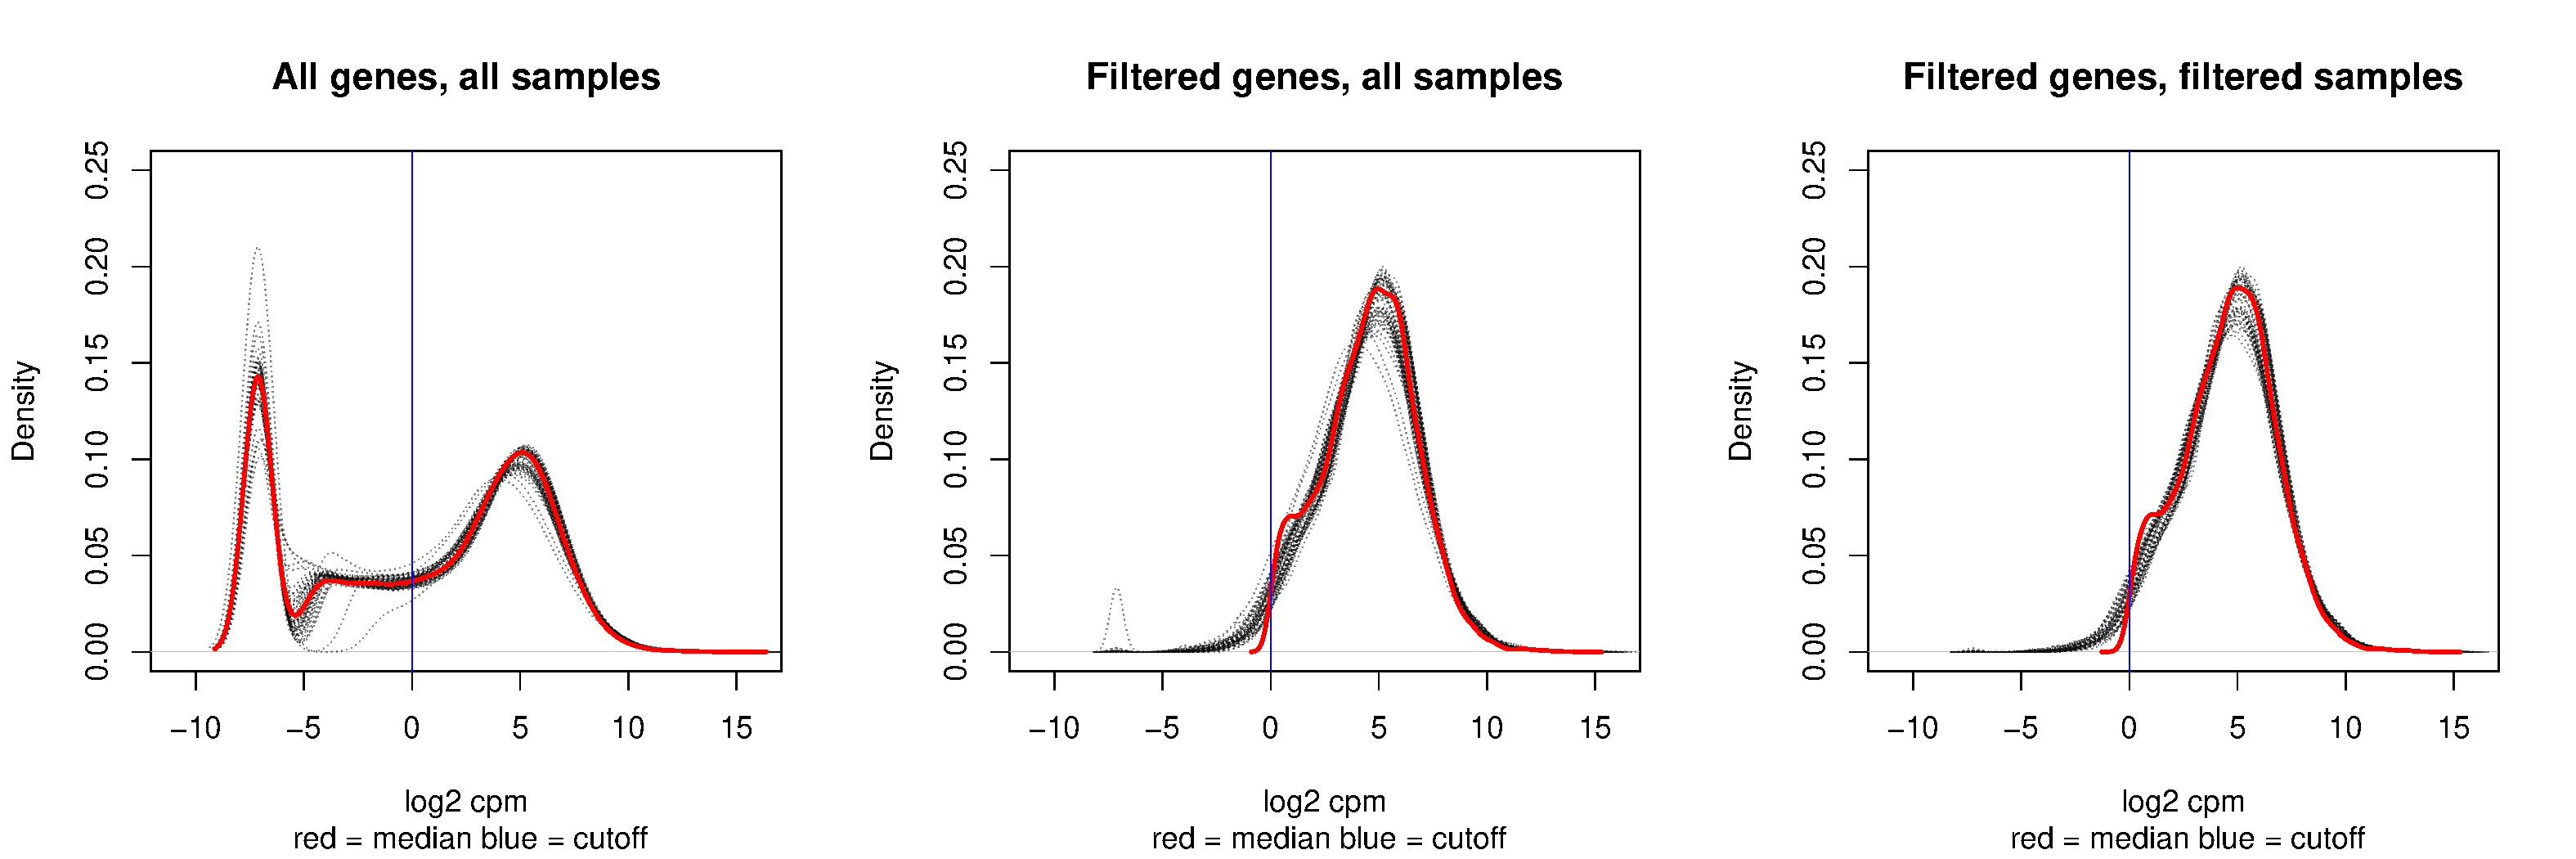
\includegraphics[width=\linewidth]{../figure/gene-exp-distribution.pdf}
\caption{
Gene expression distributions before and after filtering.
}
\label{fig:gene}
\end{figure}

\begin{figure}[ht]
\centering
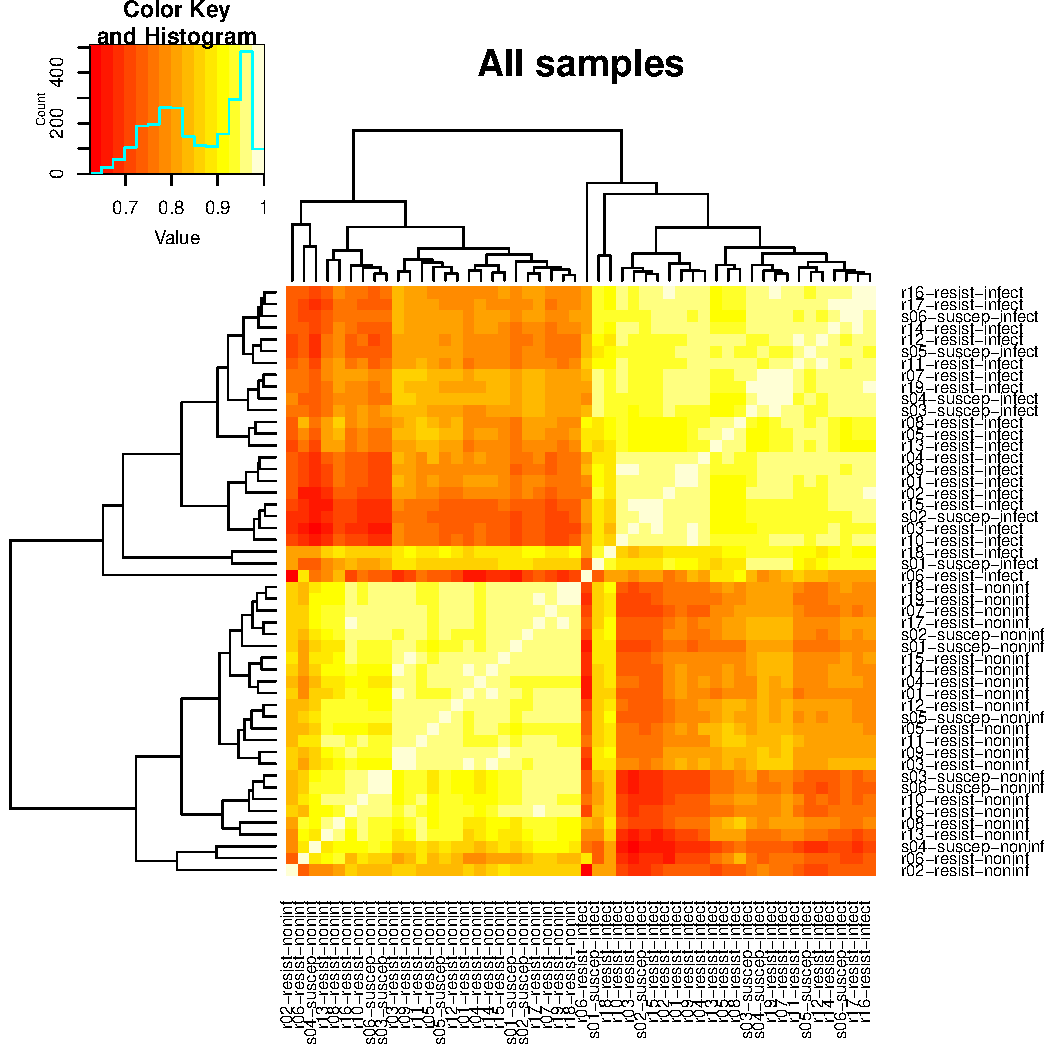
\includegraphics[width=\linewidth]{../figure/heatmap-all-samples.pdf}
\caption{
Heatmap of correlation matrix of samples.
}
\label{fig:heat-all}
\end{figure}

\begin{figure}[ht]
\centering
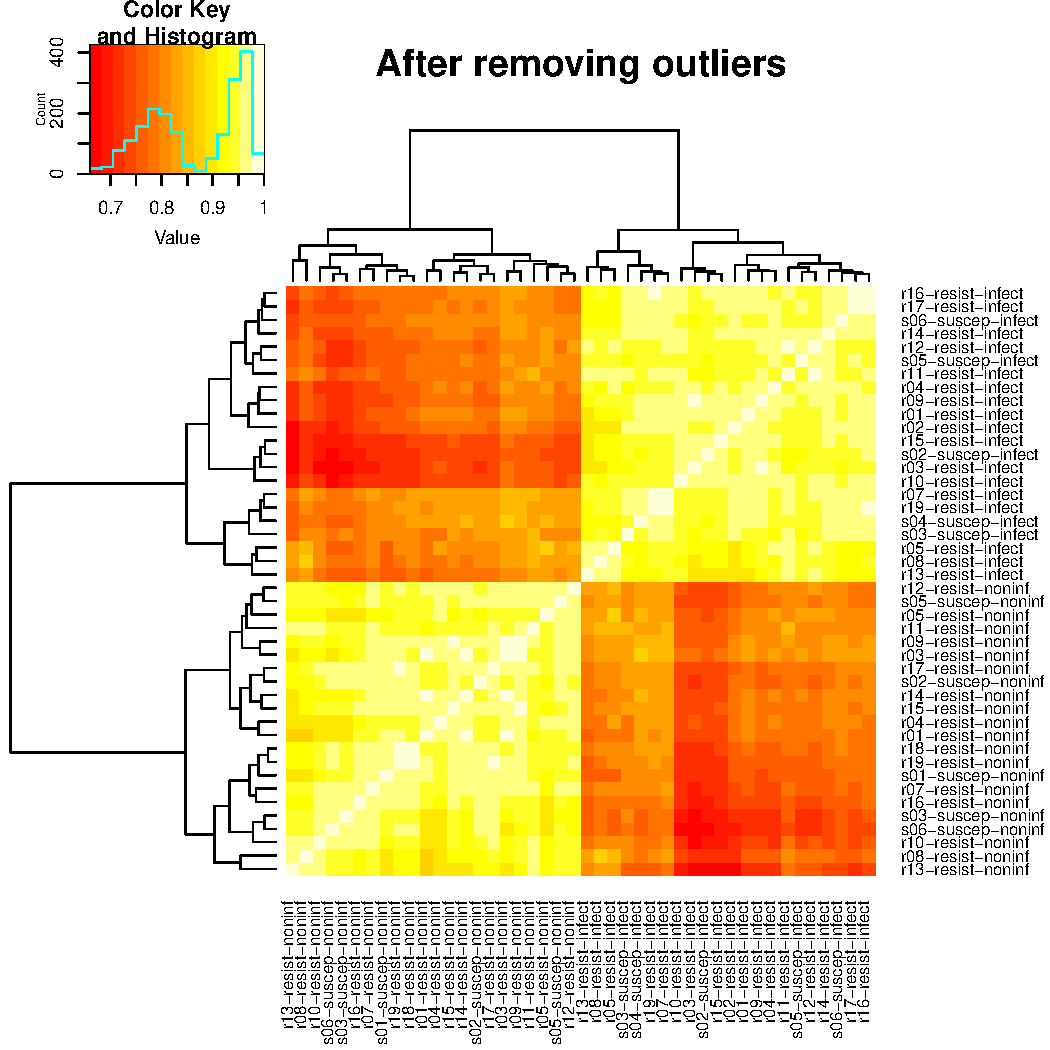
\includegraphics[width=\linewidth]{../figure/heatmap-no-outliers.pdf}
\caption{
Heatmap of correlation matrix after removing outliers.
}
\label{fig:heat-filt}
\end{figure}


\begin{figure}[ht]
\centering
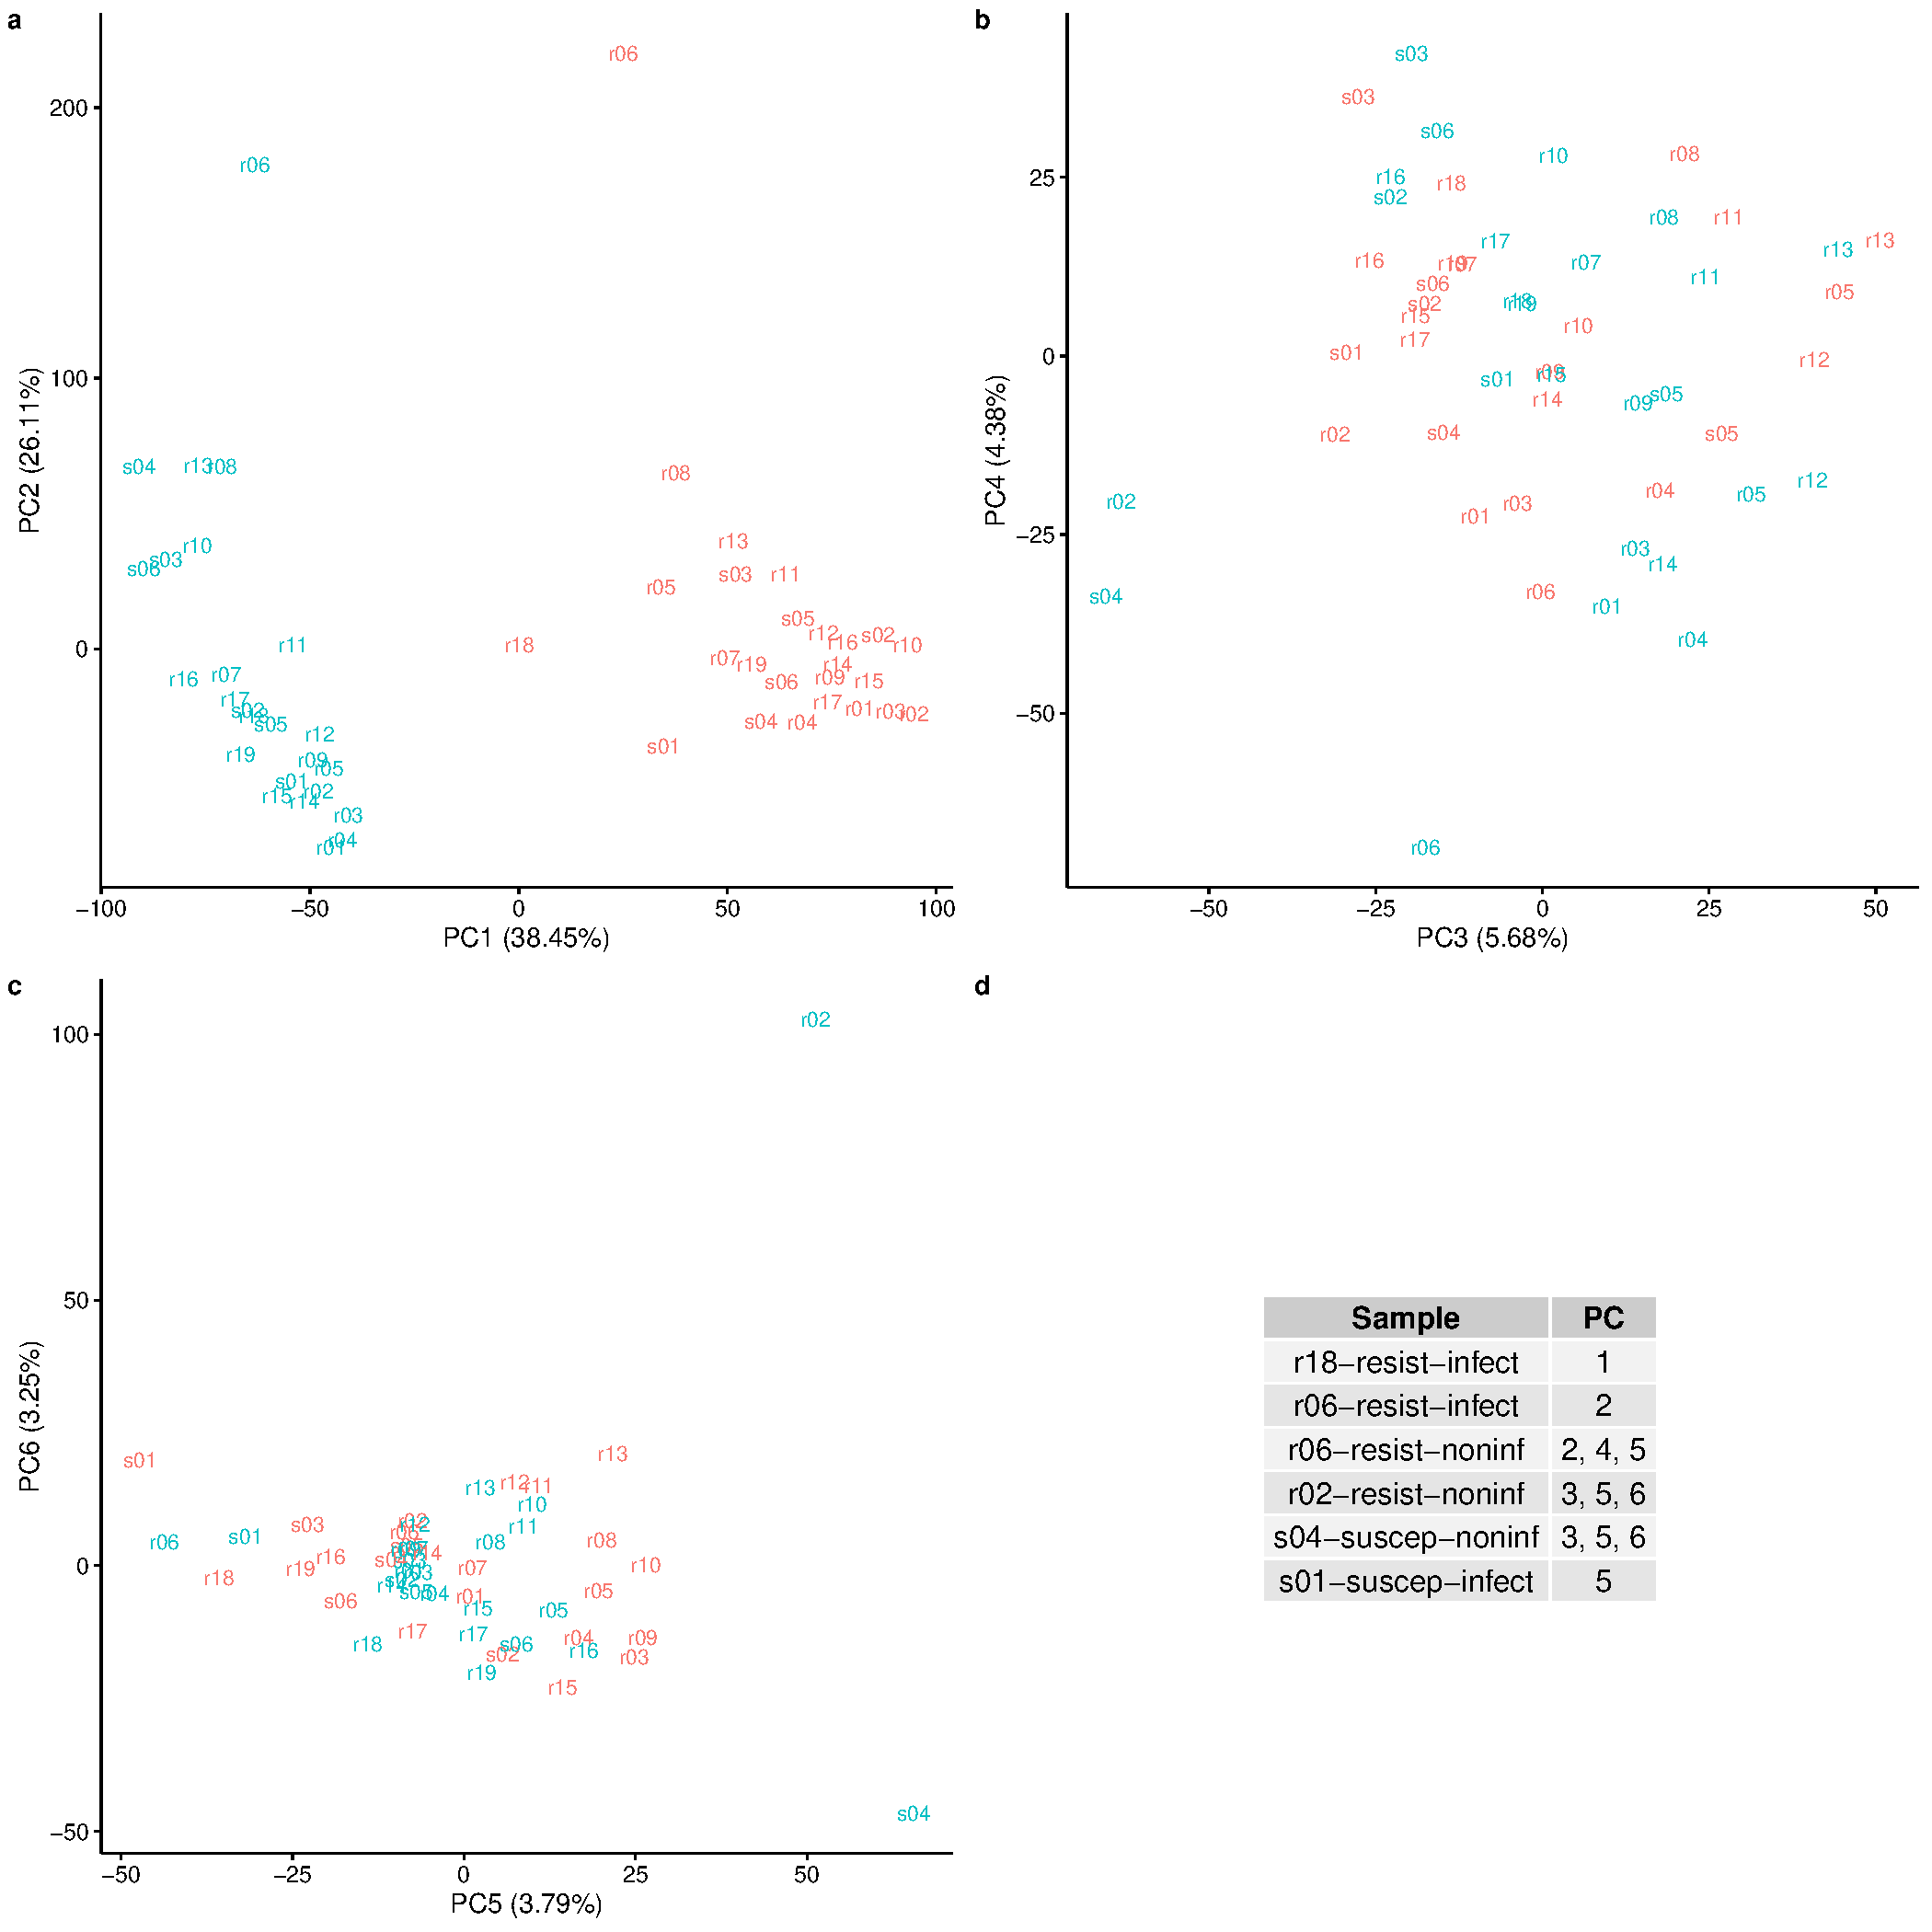
\includegraphics[width=\linewidth]{../figure/outliers.pdf}
\caption{
Remove outliers.
}
\label{fig:outliers}
\end{figure}


\begin{figure}[ht]
\centering
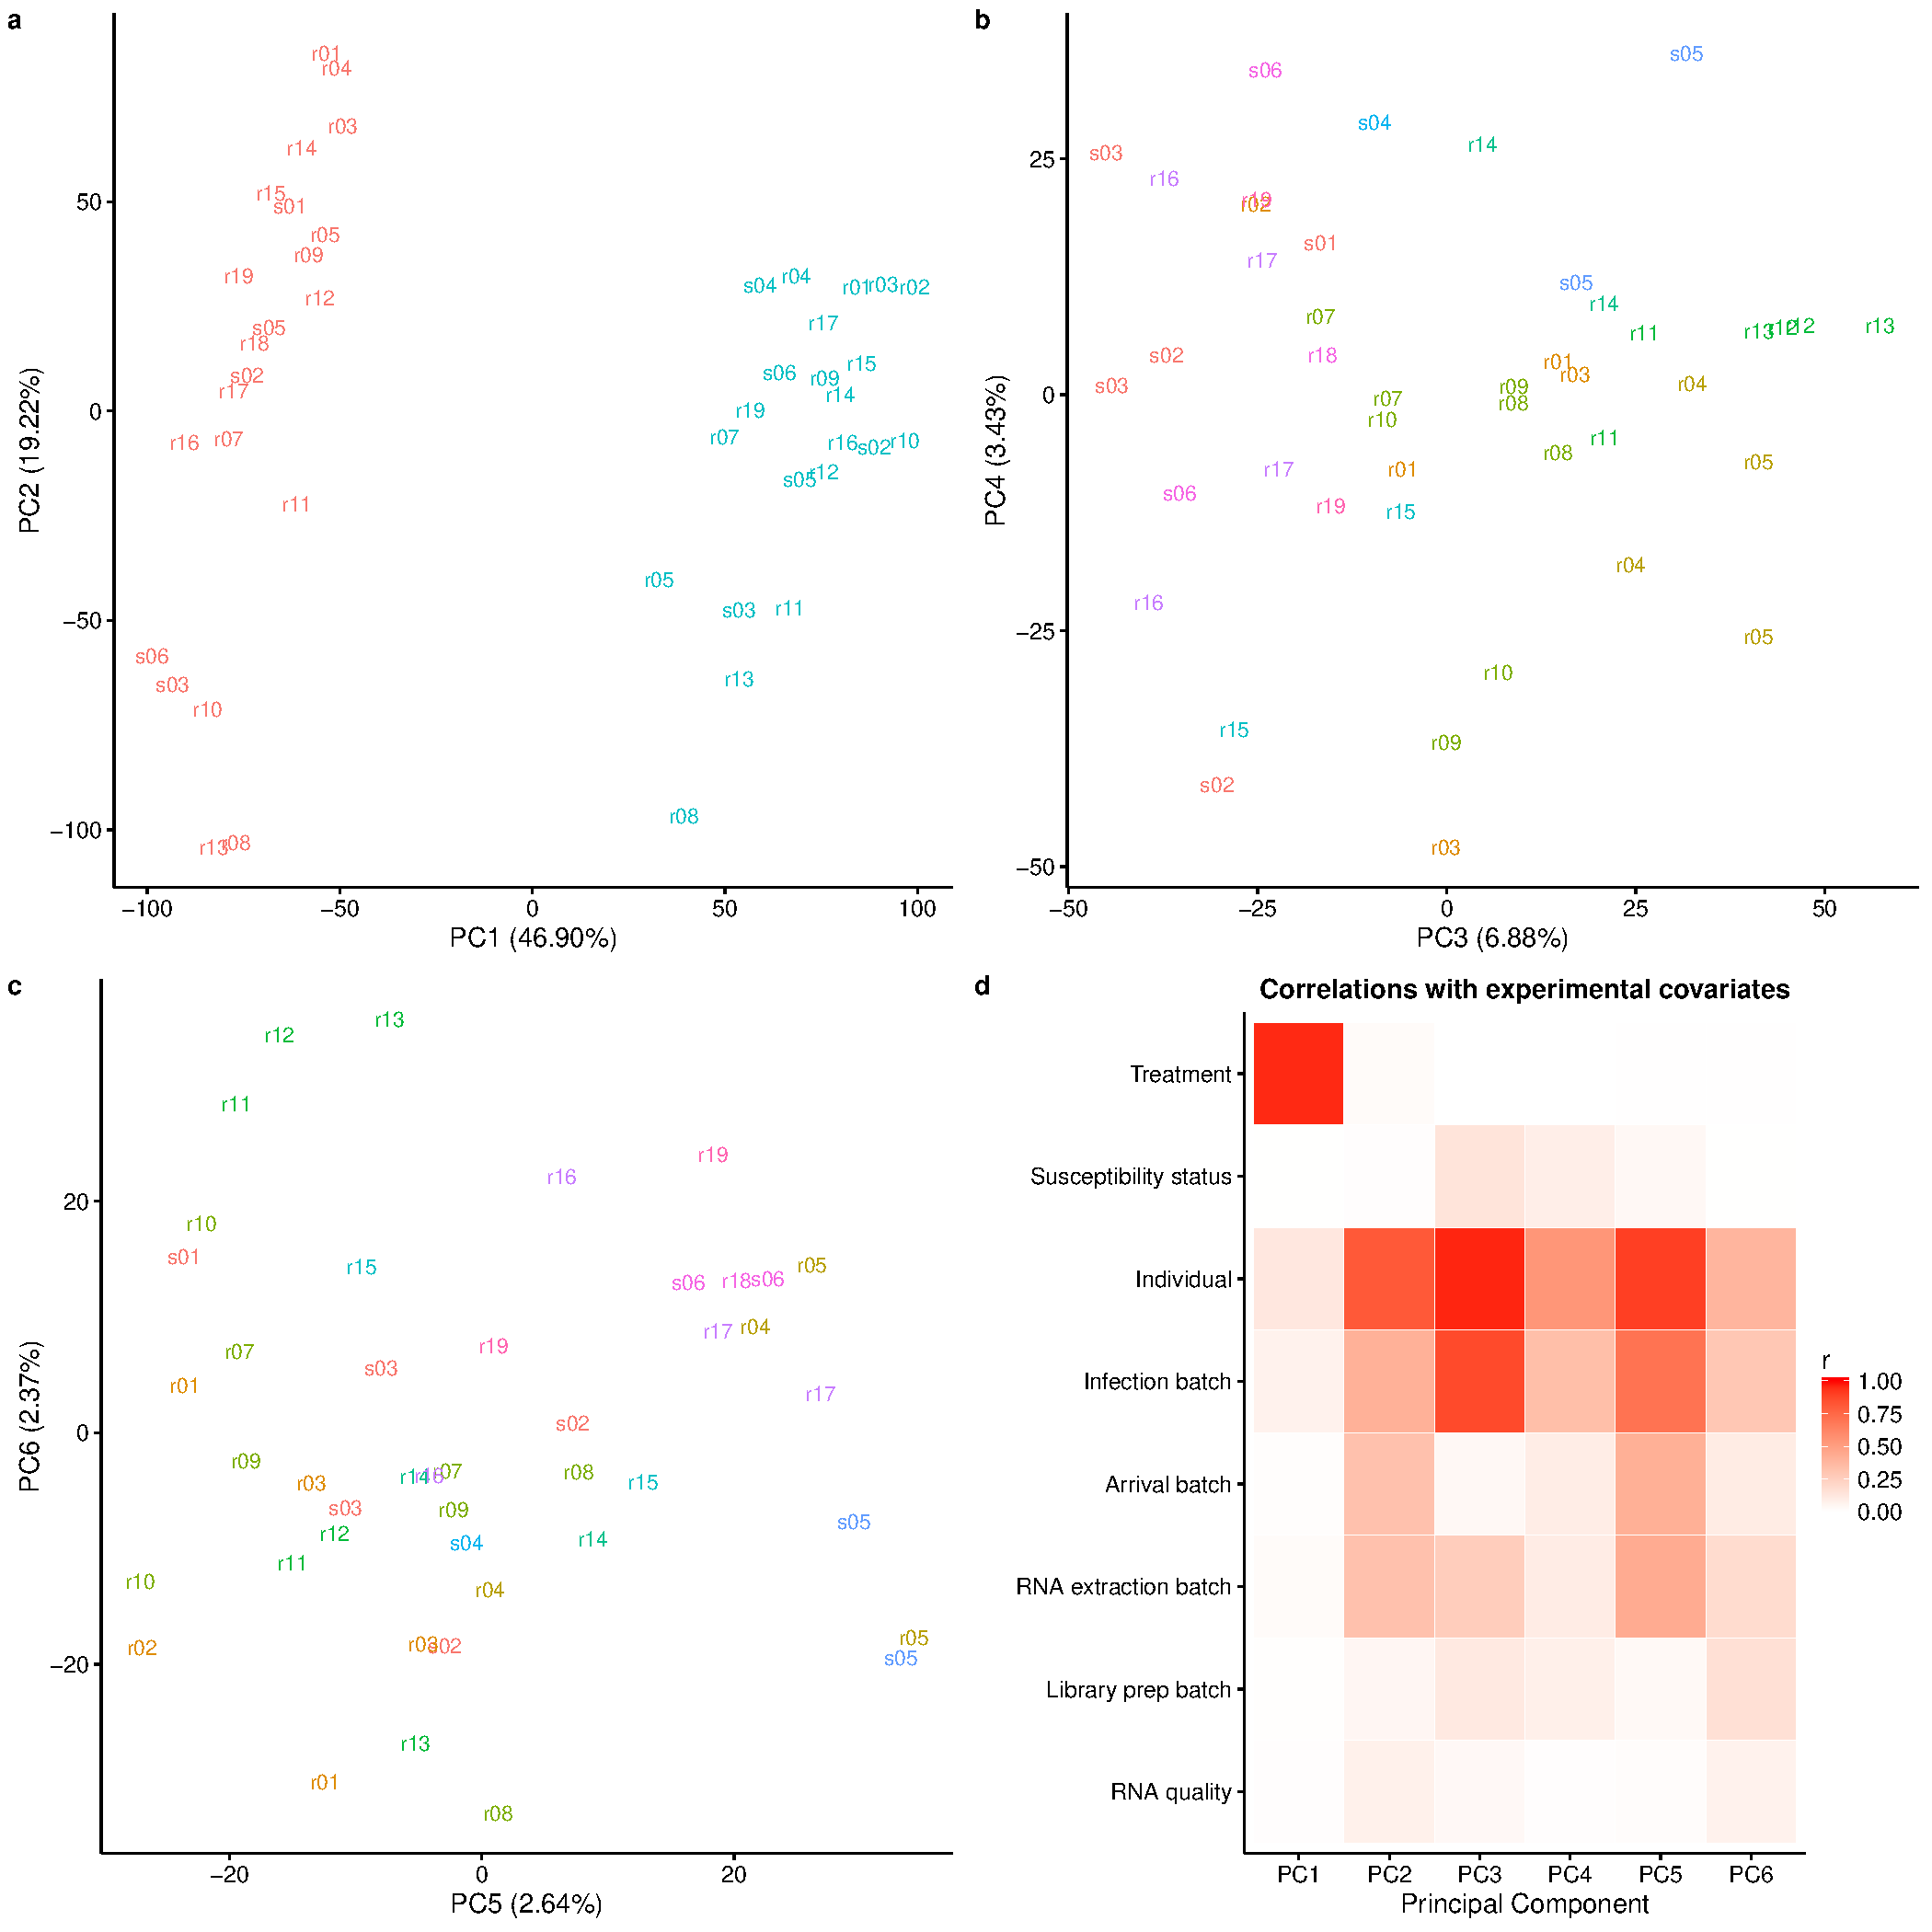
\includegraphics[width=\linewidth]{../figure/batch-pca.pdf}
\caption{
Check for technical batch effects using principal components analysis (PCA). (a) PC1 versus PC2. The text labels are the individual identifiers. Red indicates noninfected samples and blue indicates infected. (b) PC3 versus PC4. The colors indicate the different infection batches. (c) PC5 versus PC6. The colors indicate the different infection batches. (d) The Pearson correlation of PCs 1-6 with each of the recorded biological and technical covariates.
}
\label{fig:batch}
\end{figure}

\begin{figure}[ht]
\centering
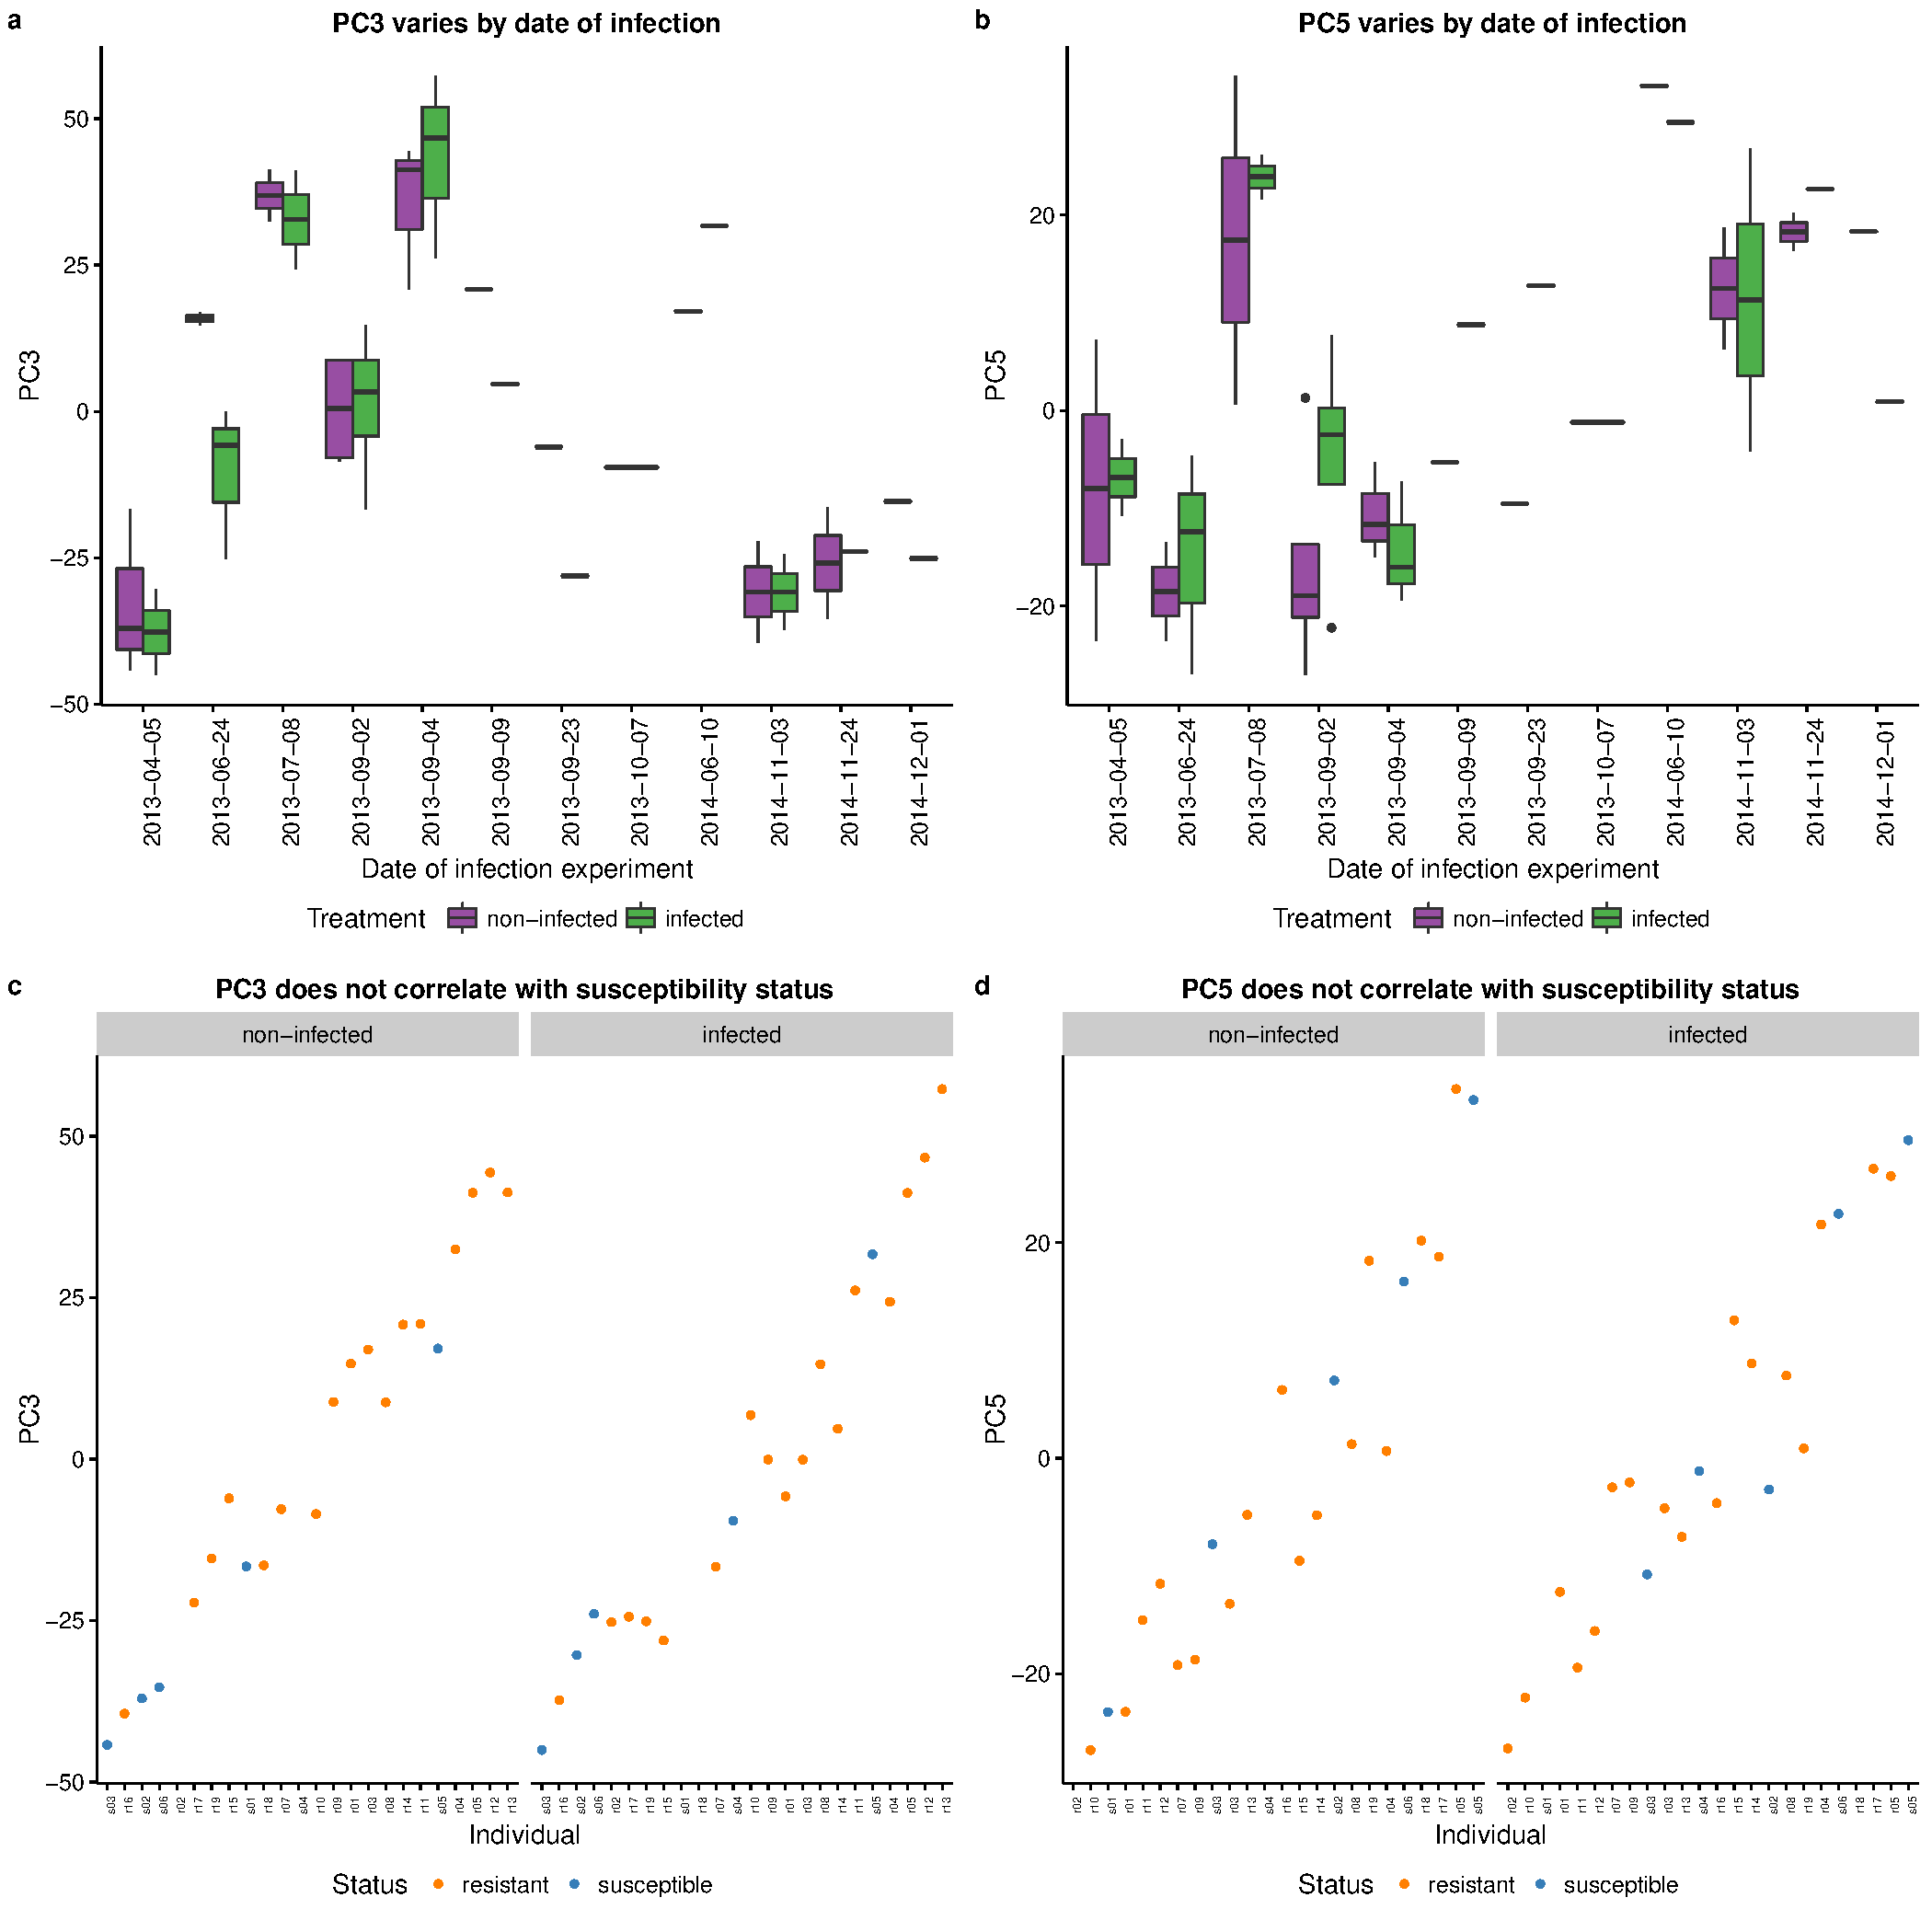
\includegraphics[width=\linewidth]{../figure/batch-infection.pdf}
\caption{
Check for confounding effect of infection batch. PC3 (a) and PC5 (b) varied by the date of infection. Importantly, however, this technical variation arising from infection batch did not correlate with the susceptibility status of the individuals (c and d).
}
\label{fig:infection}
\end{figure}

\begin{figure}[ht]
\centering
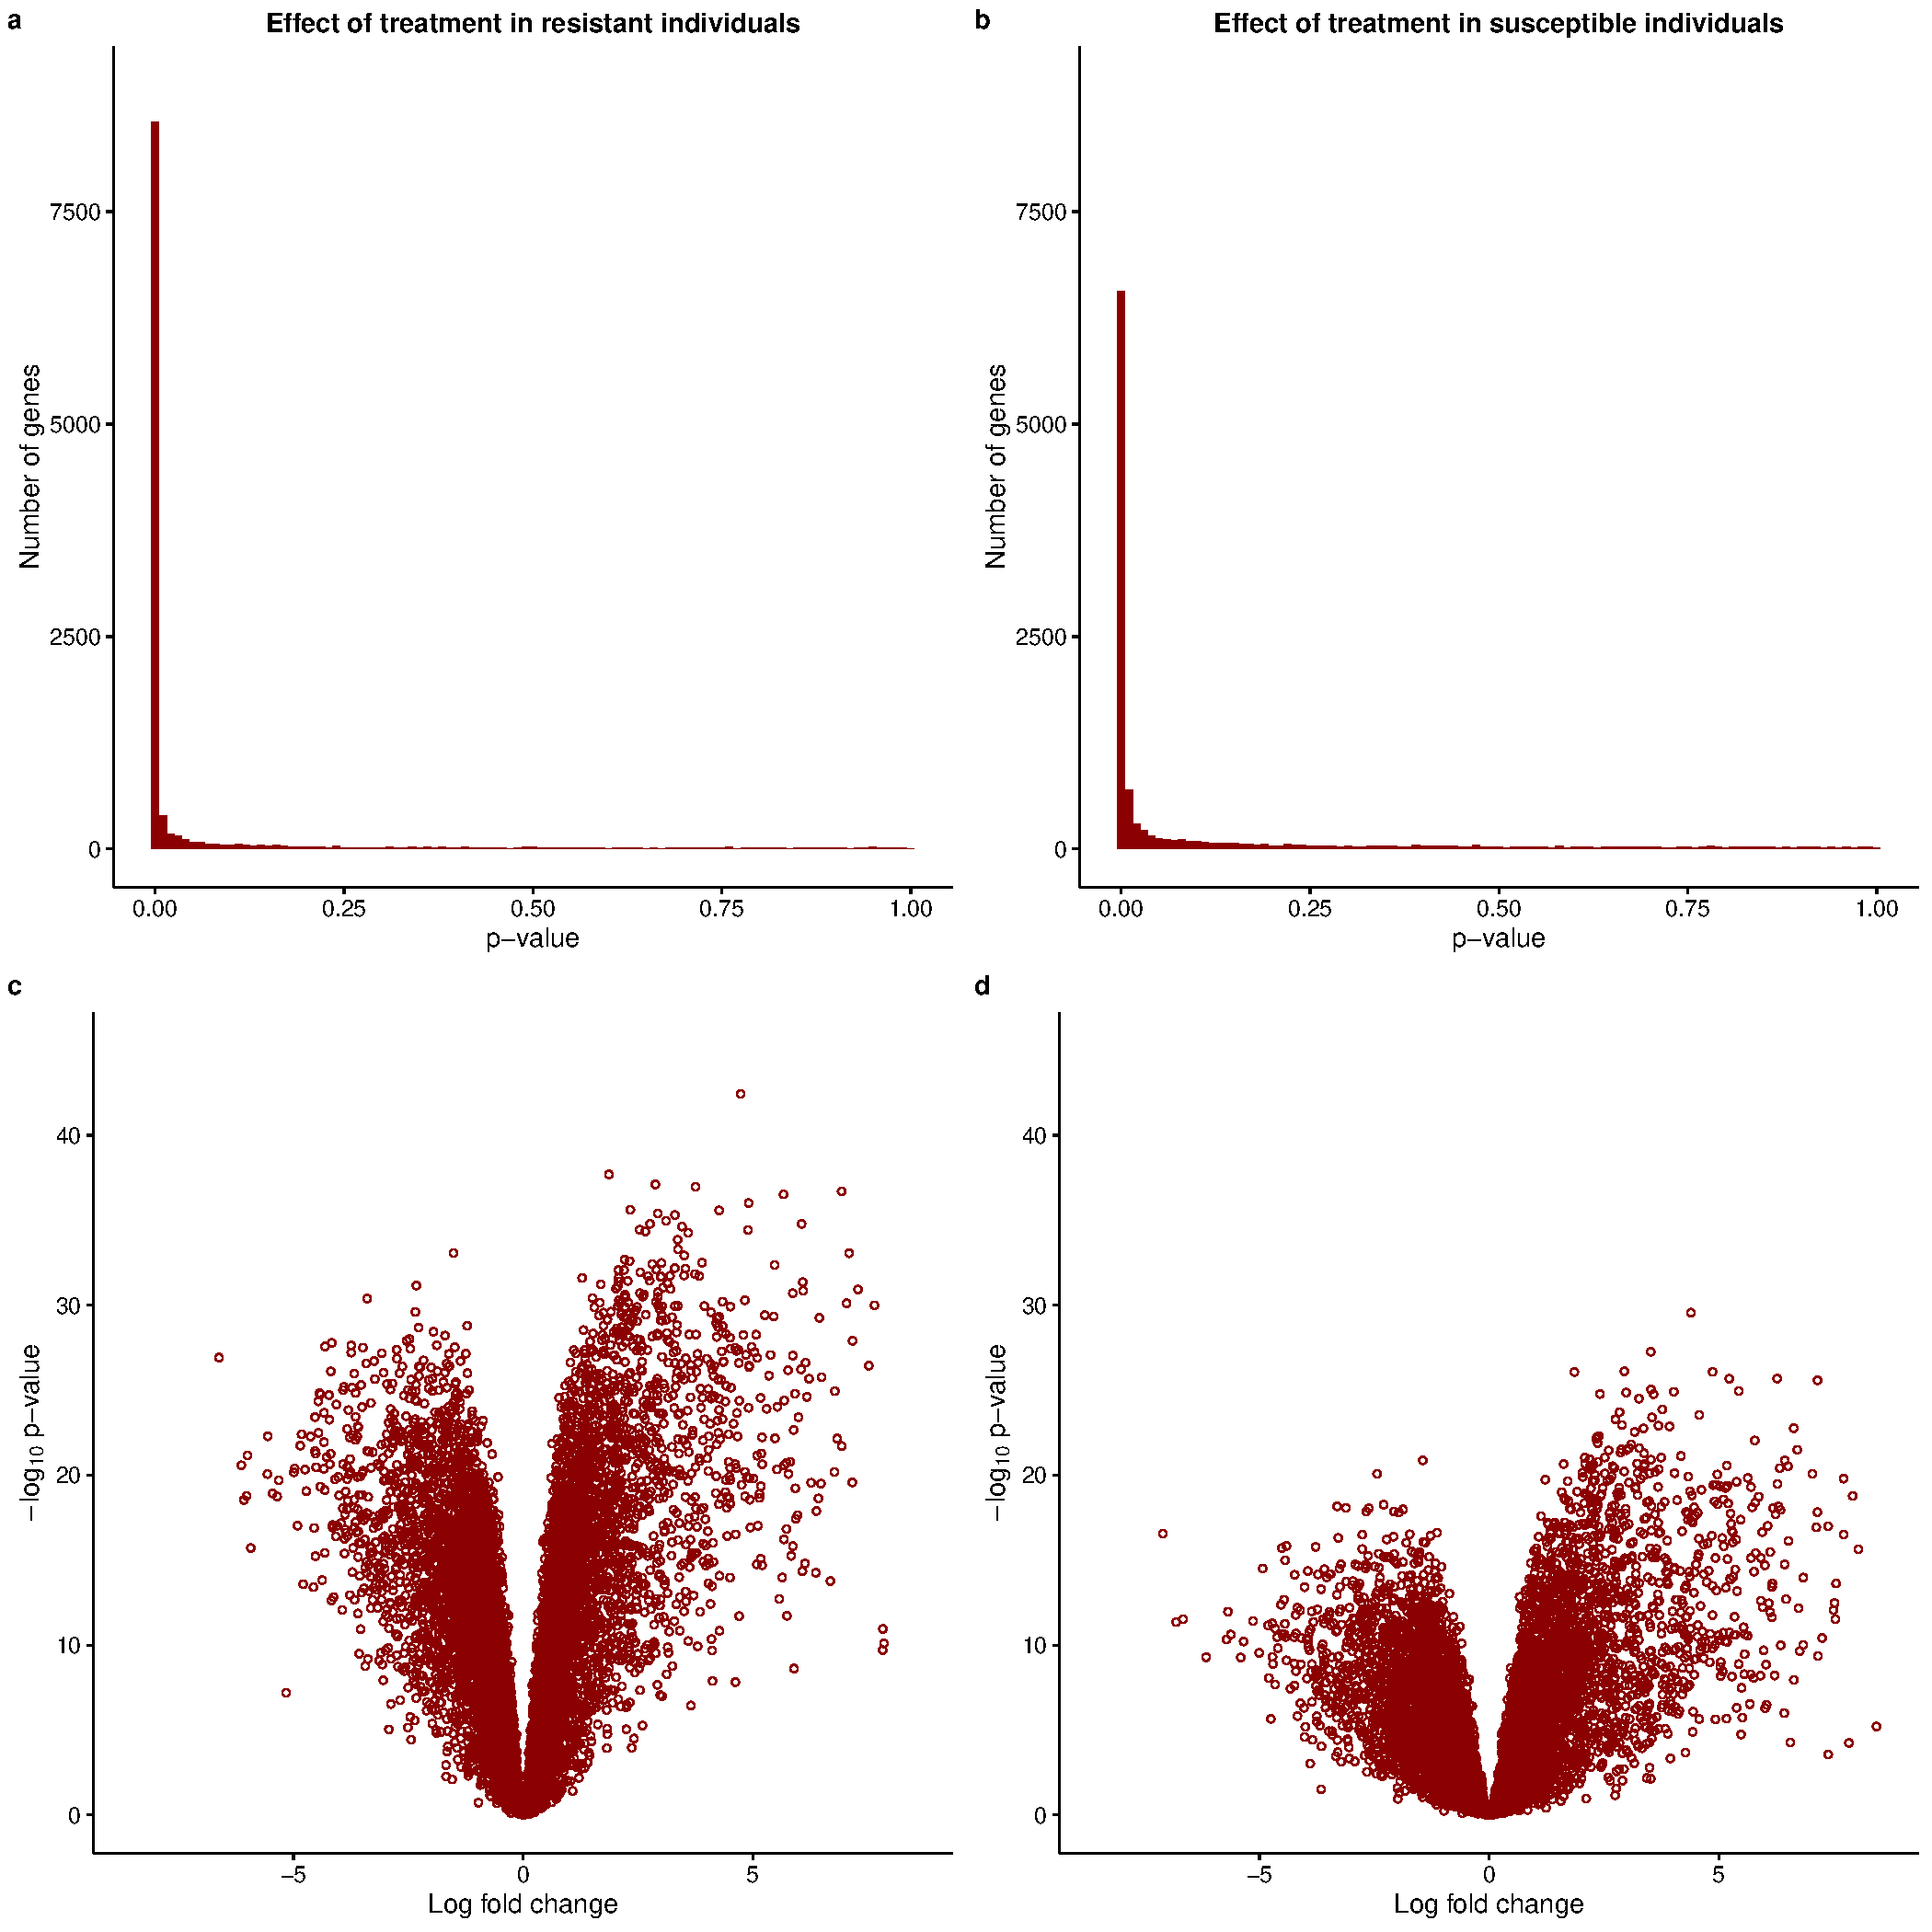
\includegraphics[width=\linewidth]{../figure/limma-supp.pdf}
\caption{
Effect of treatment.
}
\label{fig:limma-supp}
\end{figure}

\end{document}
